\documentclass[11pt,a4paper]{article}
\usepackage[utf8]{inputenc}
\usepackage{amsmath}
\usepackage{amsfonts}
\usepackage{amssymb}
\usepackage{graphicx}
\usepackage{caption}
\usepackage{subcaption}
\usepackage{comment}
\usepackage{color}
\usepackage{enumitem}
\usepackage[left=2cm,right=2cm,top=2cm,bottom=2cm]{geometry}
\graphicspath{ {./figs/} }
\author{Andrew Teta}
\title{ECEN 4532 - Lab 1}
\begin{document}
\maketitle
\section*{Introduction}
\paragraph*{} In this discussion, we will be exploring some techniques recently developed in the audio industry to organize, search, and classify large music collections. We are developing some statistical methods, along with frequency analysis to automatically characterize songs and genres.
\subsection*{Format}
\paragraph*{} Fundamentally, we begin with a '.wav' file. This is one variety of many signal encodings, generated by sampling a physical sound wave using a microphone. The microphone detects pressure differences within a medium (sound) and converts them into electrical voltages. As the voltages are converted into a digital representation, they are quantized at a sampling frequency ($fs$). Furthermore, the Nyquist sampling theorem dictates that for a signal to be represented accurately in quantized form, it must be sampled at twice the rate of the highest frequency component. For example, a dolphin can only hear sound in the range $7kHz-120kHz$, so if we want to record the sound that a dolphin would be able to hear, we have to sample at a rate $fs=240kHz$ or higher.
\paragraph*{} In this lab, we consider a small collection of music, organized by genre, in '.wav' format. Each song is sampled at $fs=11,025Hz$. Narrowing our data set even further, we will extract a 24 second sample from the middle of each song. We will then implement a short-time Fourier transform (STFT), which divides the sample into $N=512$ samples, or $46ms$ and call each 46 ms interval a 'frame'. The STFT is a good way to obtain frequency spectrum data, while maintaining a level of time-domain relevance. For the purposes of this lab, the frames will be non-overlapping.

\section{Time-domain Analysis}
\paragraph*{} We begin by extracting a $24s$ sample from the middle of each song using the python function \textit{scipy.io.wavfile.read}
\subsection{Loudness}
\paragraph{} To get a sense of 'loudness', we will compute the standard deviation over a 'frame' of size $N=512$ defined as:

\begin{align}
\sigma(n)=\sqrt{\frac{1}{N}\sum_{m=0}^{N-1} [x(nN+m)-E[x_n]]^2} && \text{with} && E[x_n]=\frac{1}{N}\sum_{m=0}^{N-1} x(nN+m)
\end{align}

\paragraph{Results} The output of the loudness calculation for one song of each genre is shown in the figures below. 

\begin{figure}[tb]
	\centering
	\begin{subfigure}[t]{\hsize}
		\centering
		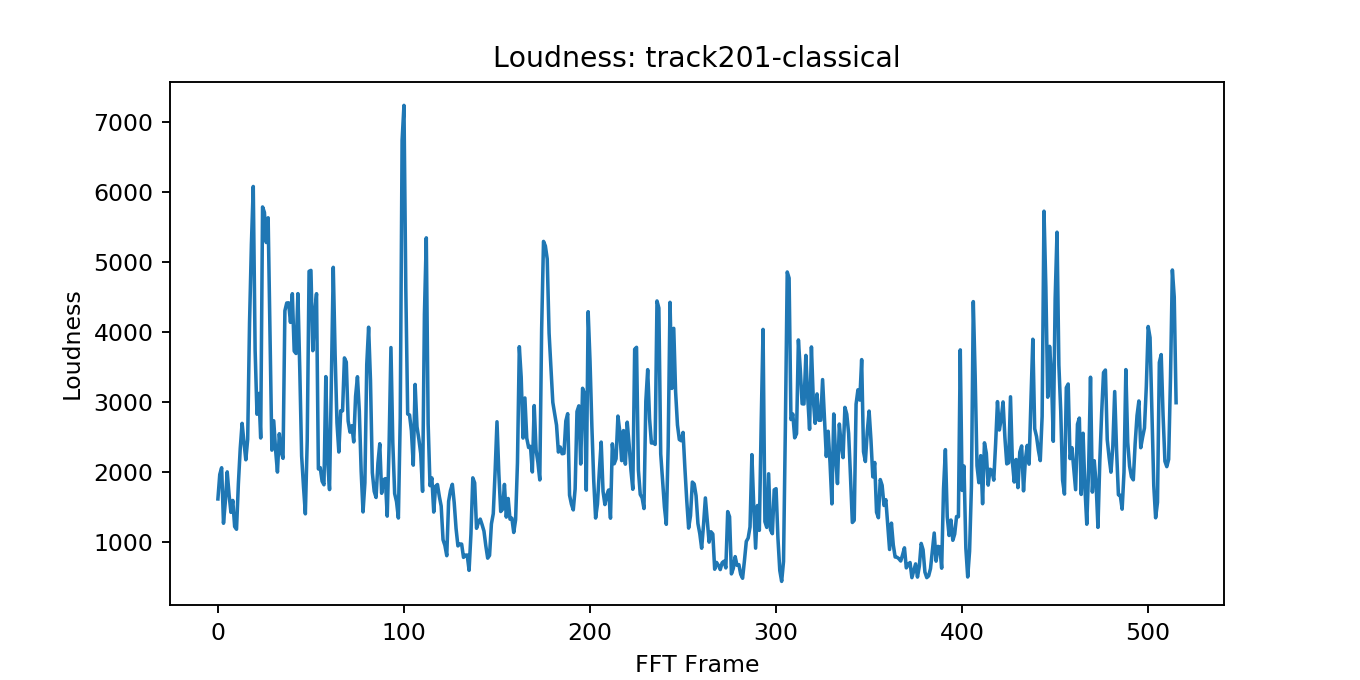
\includegraphics[width=0.9\textwidth]{loudness_track201-classical}
		\caption{'track201-classical.wav'}
		\label{fig:loudness_classical}
	\end{subfigure}
	\begin{subfigure}[t]{\hsize}
		\centering
		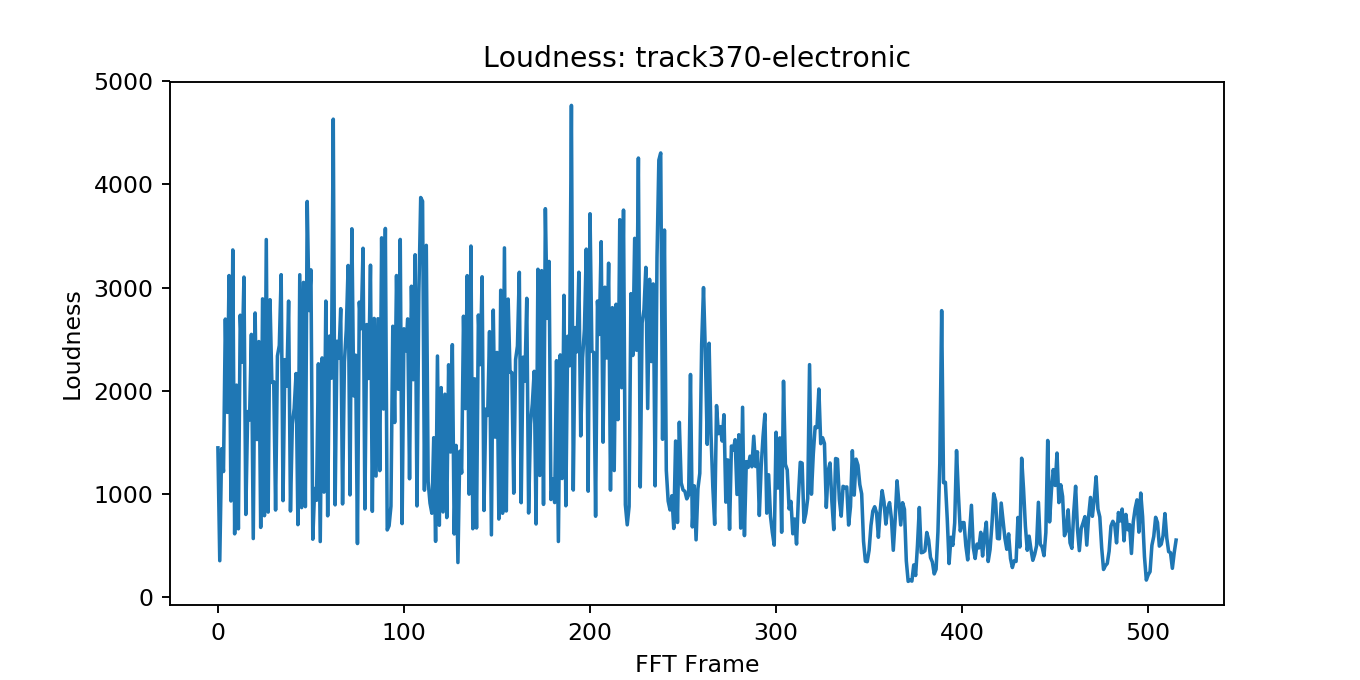
\includegraphics[width=0.9\textwidth]{loudness_track370-electronic}
		\caption{'track370-electronic.wav'}
		\label{fig:loudness_electronic}
	\end{subfigure}
	\caption{Loudness vs. frame \label{fig:loudness}}
\end{figure}
\clearpage
\begin{figure}[tb]\ContinuedFloat
	\begin{subfigure}[t]{\hsize}
		\centering
		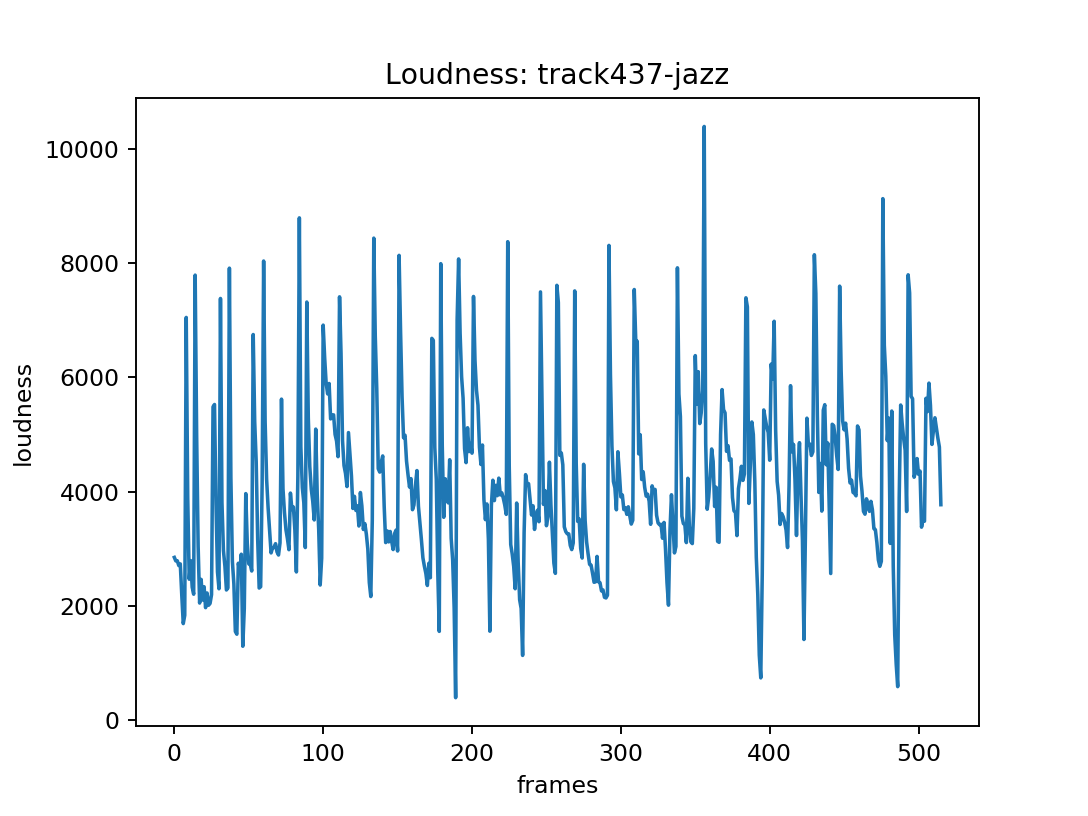
\includegraphics[width=0.9\textwidth]{loudness_track437-jazz}
		\caption{'track437-jazz.wav'}
		\label{fig:loudness_jazz}
	\end{subfigure}
	\begin{subfigure}[t]{\hsize}
		\centering
		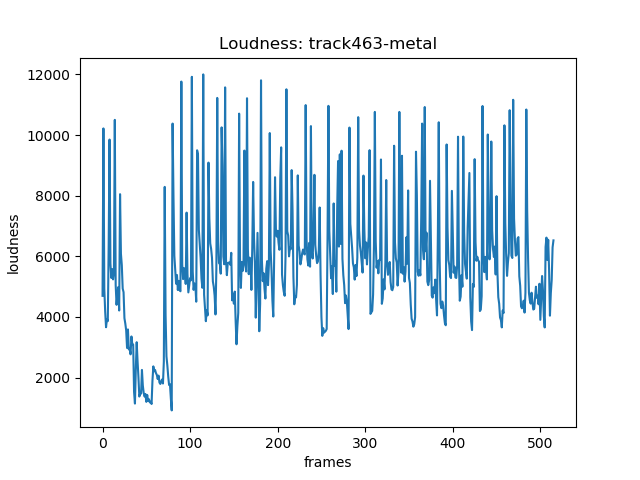
\includegraphics[width=0.9\textwidth]{loudness_track463-metal}
		\caption{'track463-metal.wav'}
		\label{fig:loudness_metal}
	\end{subfigure}
	\caption{Loudness vs. frame}
\end{figure}
\clearpage
\begin{figure}[tb]\ContinuedFloat
	\begin{subfigure}[t]{\hsize}
		\centering
		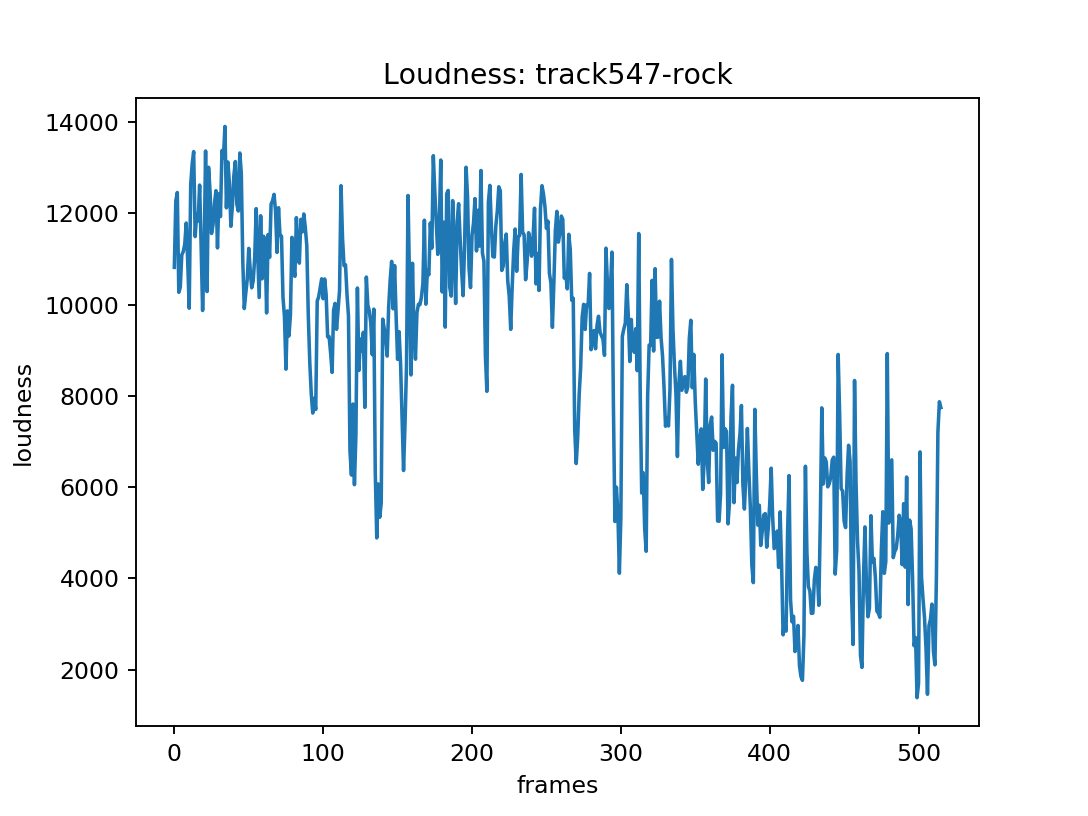
\includegraphics[width=0.9\textwidth]{loudness_track547-rock}
		\label{fig:loudness_rock}
		\caption{'track547-rock.wav'}
	\end{subfigure}
	\begin{subfigure}[t]{\hsize}
		\centering
		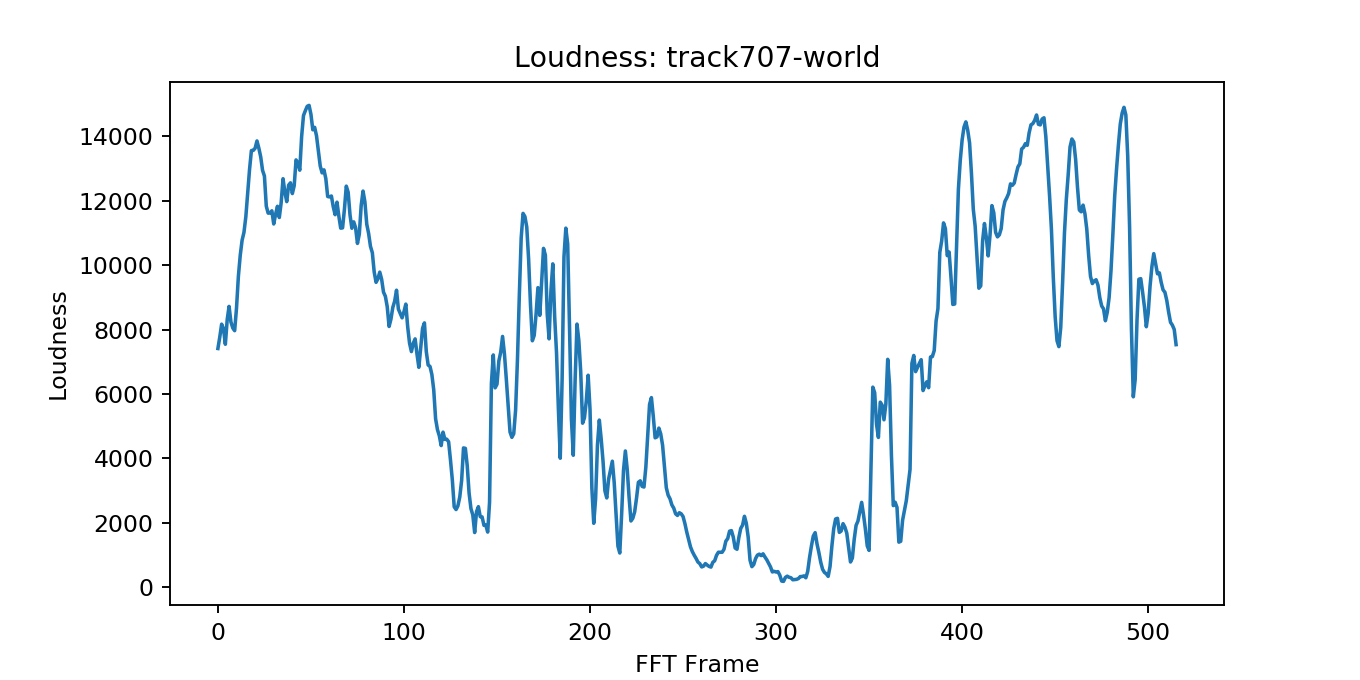
\includegraphics[width=0.9\textwidth]{loudness_track707-world}
		\caption{'track707-world.wav'}
		\label{fig:loudness_world}
	\end{subfigure}
\caption{Loudness vs. frame}
\end{figure}
\clearpage

\paragraph*{Comments} While each of the plots in figure \ref{fig:loudness} has its own characteristics, loudness is not the best tool for characterizing genres. Figure \ref{fig:loudness_electronic} shows the uniformity of the track over time and contrasts with figure \ref{fig:loudness_world} as well as figure \ref{fig:loudness_classical}, however it would be hard to distinguish between figure \ref{fig:loudness_electronic} and figure \ref{fig:loudness_metal}. However, these plots do give a good sense of the progression of each song during the sample considered.

\subsection{Zero Crossing Rate}
\paragraph*{} The zero crossing rate (ZCR) is the average number of times the audio signal crosses the zero amplitude line per unit time. It is related to pitch height and correlated to the noise in the signal. For this lab, ZCR is defined as:

\begin{equation}
ZCR(n)=\frac{1}{N-1}\sum_{m=1}^{N-1}\frac{1}{2}|sgn(x(nN+m))-sgn(x(nN+m-1))|.
\end{equation}

\paragraph{Results} Again, we display the output of computed ZCR for one track of each genre in the figures below.

\begin{figure}[tb]
	\centering
	\begin{subfigure}[t]{\hsize}
		\centering
		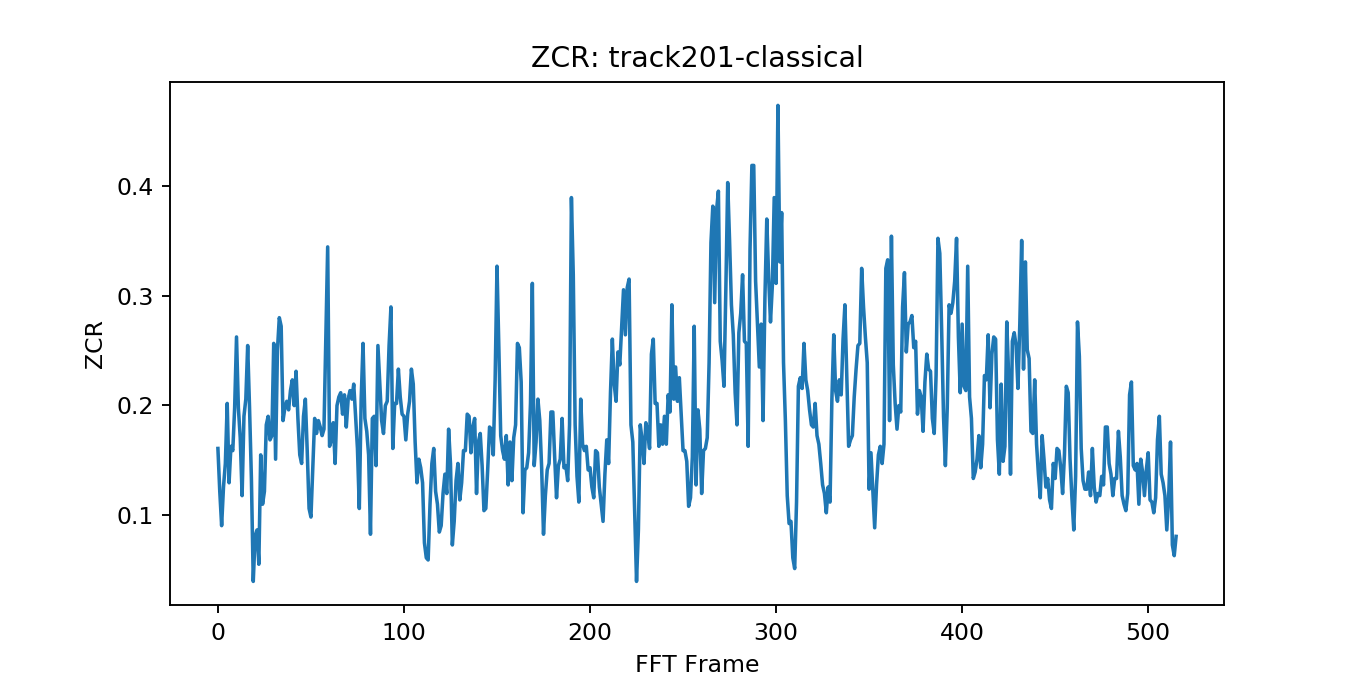
\includegraphics[width=0.9\textwidth]{zcr_track201-classical}
		\caption{'track201-classical.wav'}
		\label{fig:zcr_classical}
	\end{subfigure}
	\begin{subfigure}[t]{\hsize}
		\centering
		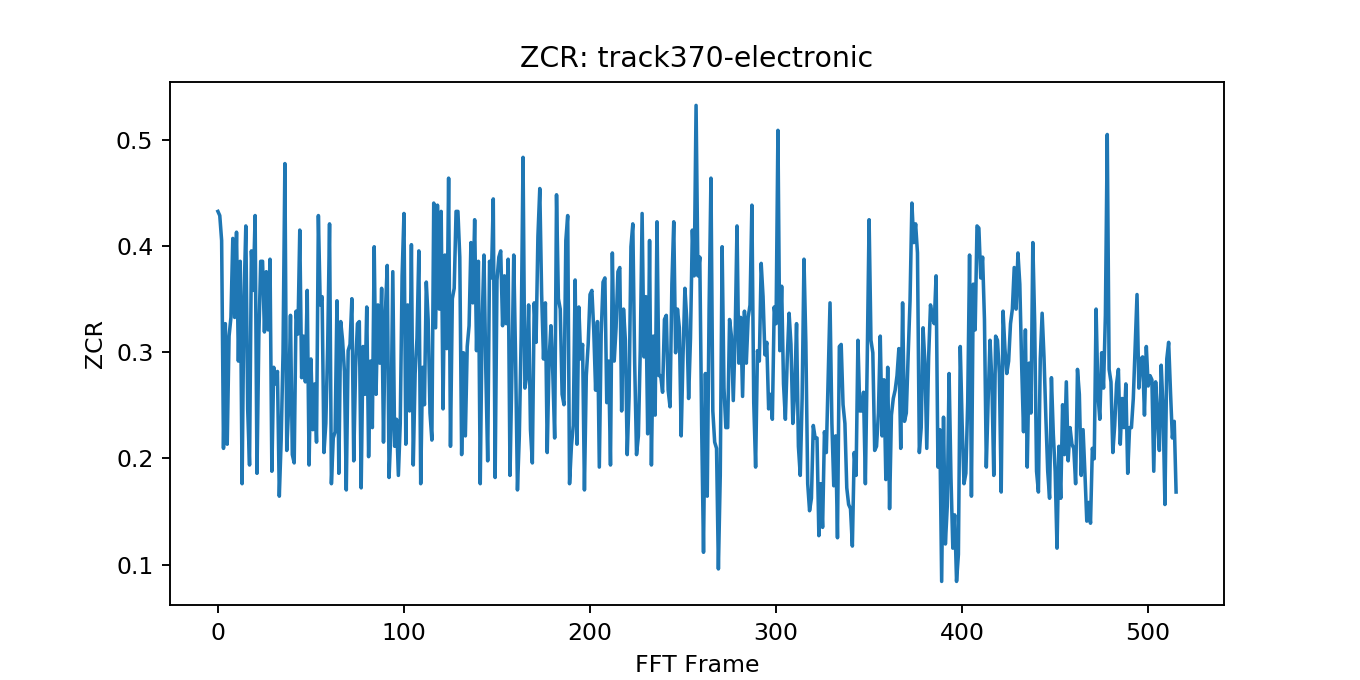
\includegraphics[width=0.9\textwidth]{zcr_track370-electronic}
		\caption{'track370-electronic.wav'}
		\label{fig:zcr_electronic}
	\end{subfigure}
	\caption{Loudness vs. frame \label{fig:zcr}}
\end{figure}
\clearpage
\begin{figure}[tb]\ContinuedFloat
	\begin{subfigure}[t]{\hsize}
		\centering
		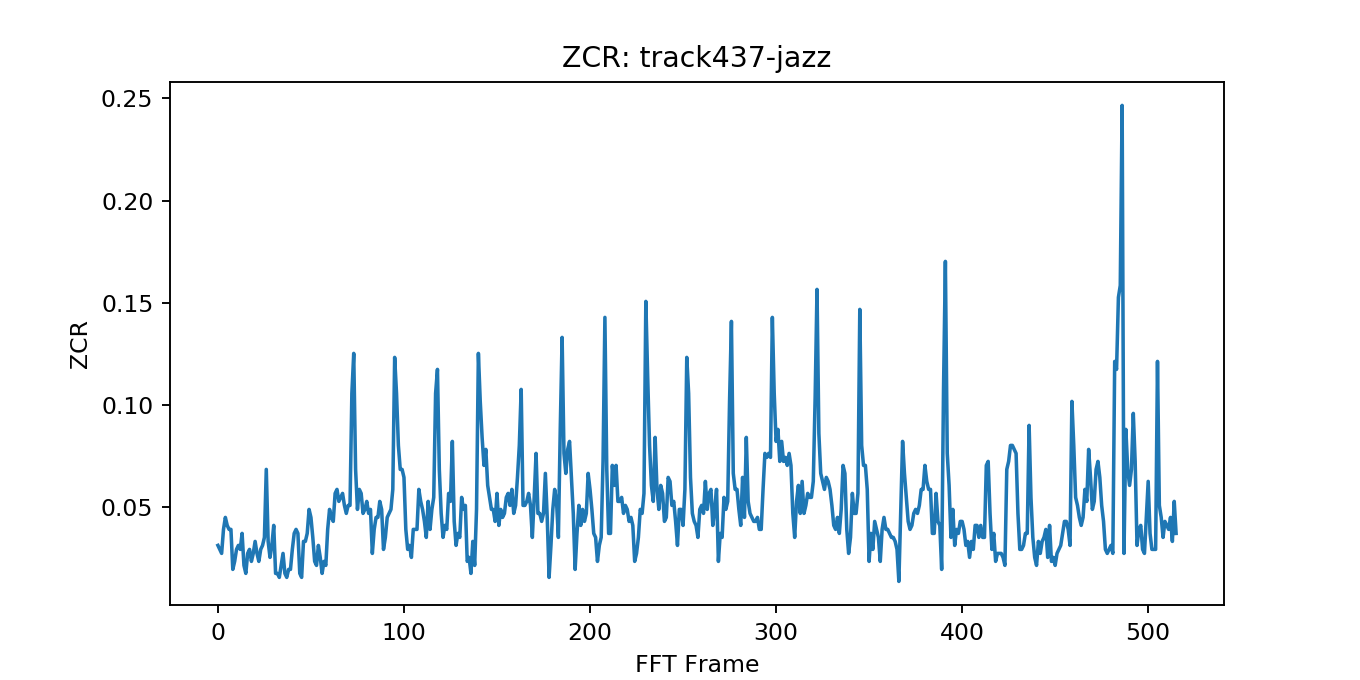
\includegraphics[width=0.9\textwidth]{zcr_track437-jazz}
		\caption{'track437-jazz.wav'}
		\label{fig:zcr_jazz}
	\end{subfigure}
	\begin{subfigure}[t]{\hsize}
		\centering
		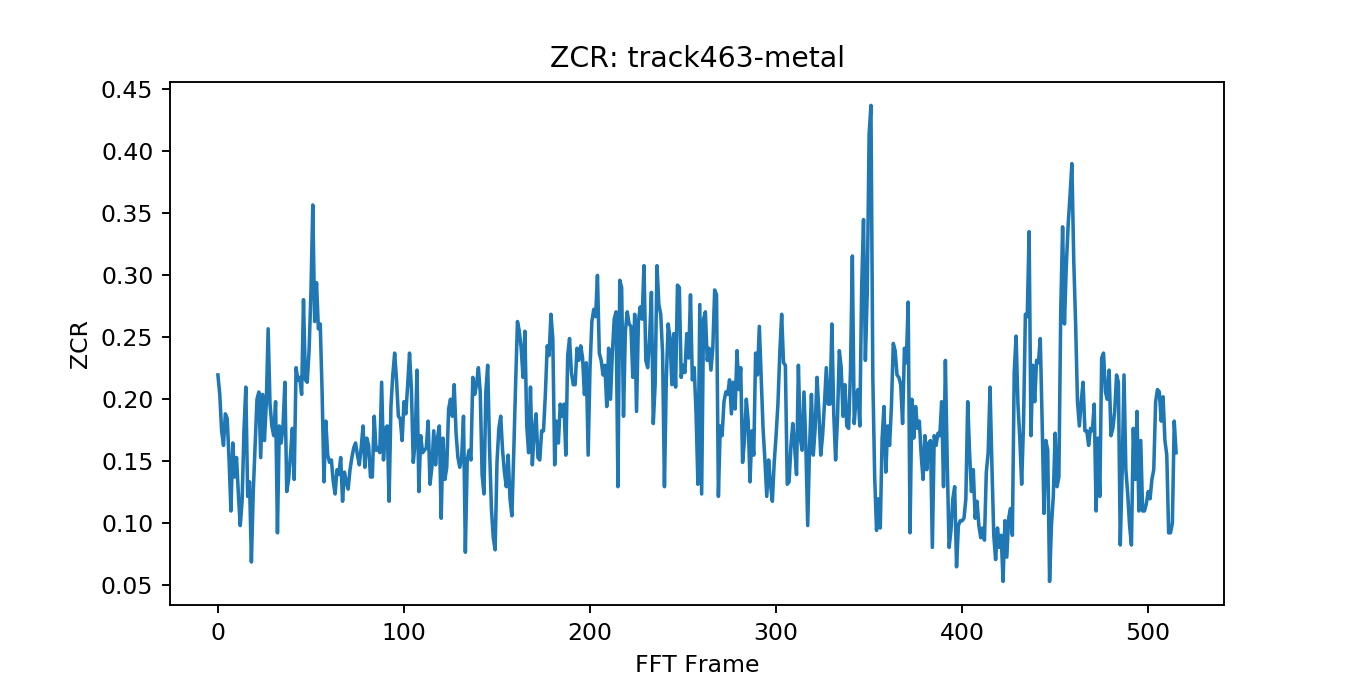
\includegraphics[width=0.9\textwidth]{zcr_track463-metal}
		\caption{'track463-metal.wav'}
		\label{fig:zcr_metal}
	\end{subfigure}
	\caption{Loudness vs. frame}
\end{figure}
\clearpage
\begin{figure}[tb]\ContinuedFloat
	\begin{subfigure}[t]{\hsize}
		\centering
		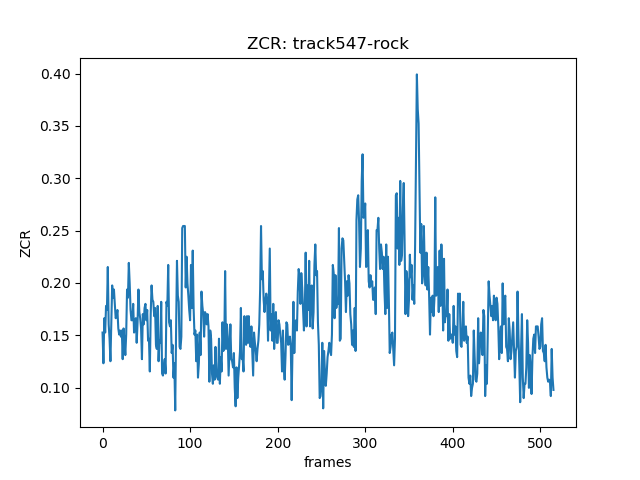
\includegraphics[width=0.9\textwidth]{zcr_track547-rock}
		\caption{'track547-rock.wav'}
		\label{fig:zcr_rock}
	\end{subfigure}
	\begin{subfigure}[t]{\hsize}
		\centering
		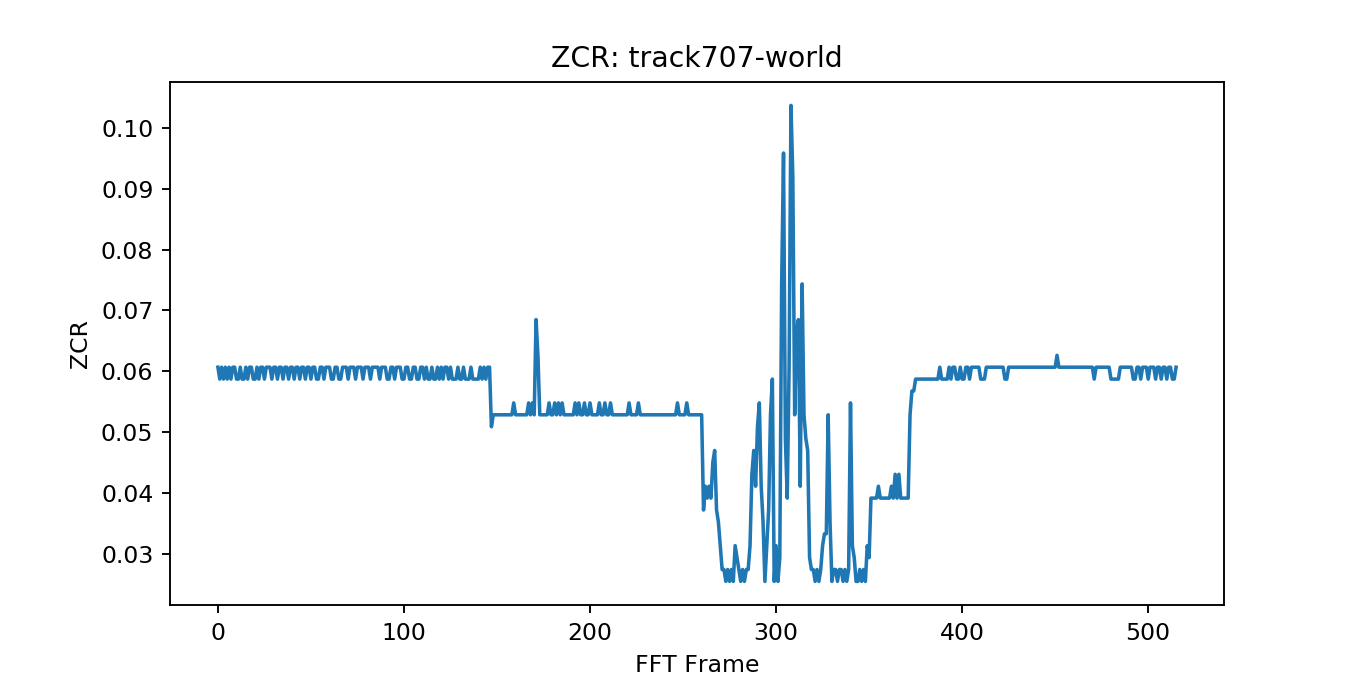
\includegraphics[width=0.9\textwidth]{zcr_track707-world}
		\caption{'track707-world.wav'}
		\label{fig:zcr_world}
	\end{subfigure}
	\caption{Loudness vs. frame}
\end{figure}
\clearpage

\paragraph{Comments} From the plots in figure \ref{fig:zcr} we can definitely see some variability between genres. For example, the world track in \ref{fig:zcr_world} is easily distinguishable, however most of the other tracks are similar enough that this is also not likely a good measurement for classifying genre. This can be supported by the similarity between jazz (\ref{fig:zcr_jazz}) and rock (\ref{fig:zcr_rock}).

\section{Spectral Analysis}
\paragraph*{} Sound, by nature is made up of many different frequencies or notes of different pitch. Thus it is natural to analyze audio in the spectral (frequency) domain. 
\paragraph{Method} As discussed in the introduction, we will accomplish our spectral analysis using a STFT, which decomposes short-time frames of a signal into discrete frequency bins, maintaining some time-domain relevance within the spectral domain. Then, we will perform some statistical analysis on the signal in an attempt to characterize some songs.
\paragraph*{} Rather than directly splitting each of our $N=512$ frames, we will convolve (a fancy term for multiplication in the frequency domain) a taper window, $w$, with the signal and take the Fourier transform (FT). Since the signal is real, and we are concerned only with the magnitude, we will compute the FT of only half of the frequency spectrum to arrive at $N/2=256$ frequency bins for each of our $N=512$ frames. Finally, for the purposes of this analysis, we are interested in the power spectrum of the original song, so we take the magnitude squared (i.e. $|X_n(k)|^2$, as a function of the frame index $n$ and frequency index $k$).
\paragraph*{} To give some motivation for the taper window, $w$, we will derive the theoretical discrete-time Fourier transform (DTFT) for a given signal $x[n]$ where,

\begin{align*}
x[n] &= 1, && -N/2 \leq n \leq N/2 \\
x[n] &= 0, && \text{else}
\end{align*}

Recall the definition of the DTFT.

\begin{equation} \label{eq:dtft}
X(\omega)=\sum_{n=-\infty}^{\infty} x[n]e^{-j\omega n}.
\end{equation}

Since $x[n]\neq 0$ over only a subset of values in the DTFT range, equation \eqref{eq:dtft} becomes,

\begin{align*}
X(\omega) &= \sum_{n=-N/2}^{N/2} x[n]e^{-j\omega n} \\
		  &= \sum_{n=-N/2}^{N/2} e^{-j\omega n} 
\end{align*}

\clearpage

\subsection{Spectrogram} As promised, we will be implementing a STFT. In Python, we will use the $scipy.signal.spectrogram$ function to automate this. However, we first need a window. For this, we will use the library function, $scipy.signal.get\_window$ which allows us to quickly generate taper windows of the same size as our STFT frames. There are many choices of windows, but we will look at the 'Hann' and 'Blackman' windows. See figure \ref{fig:windows}.

\begin{figure}[ht]
	\centering
	\begin{subfigure}[t]{\hsize}
	\centering
		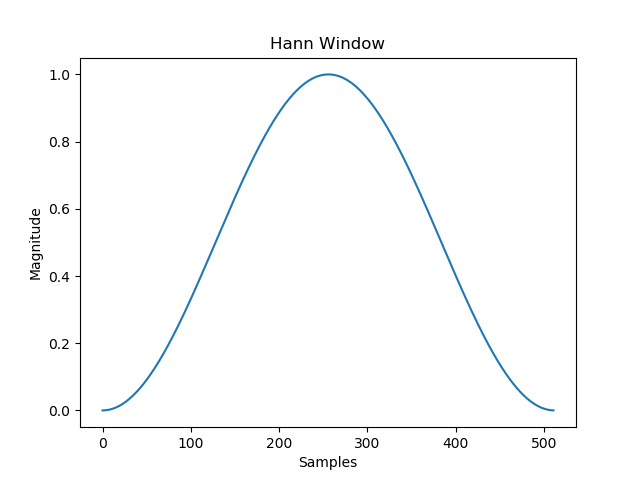
\includegraphics[width=0.6\textwidth]{hann}
		\caption{Hann window}
		\label{fig:hann}
	\end{subfigure}
	\begin{subfigure}[t]{\hsize}
		\centering
		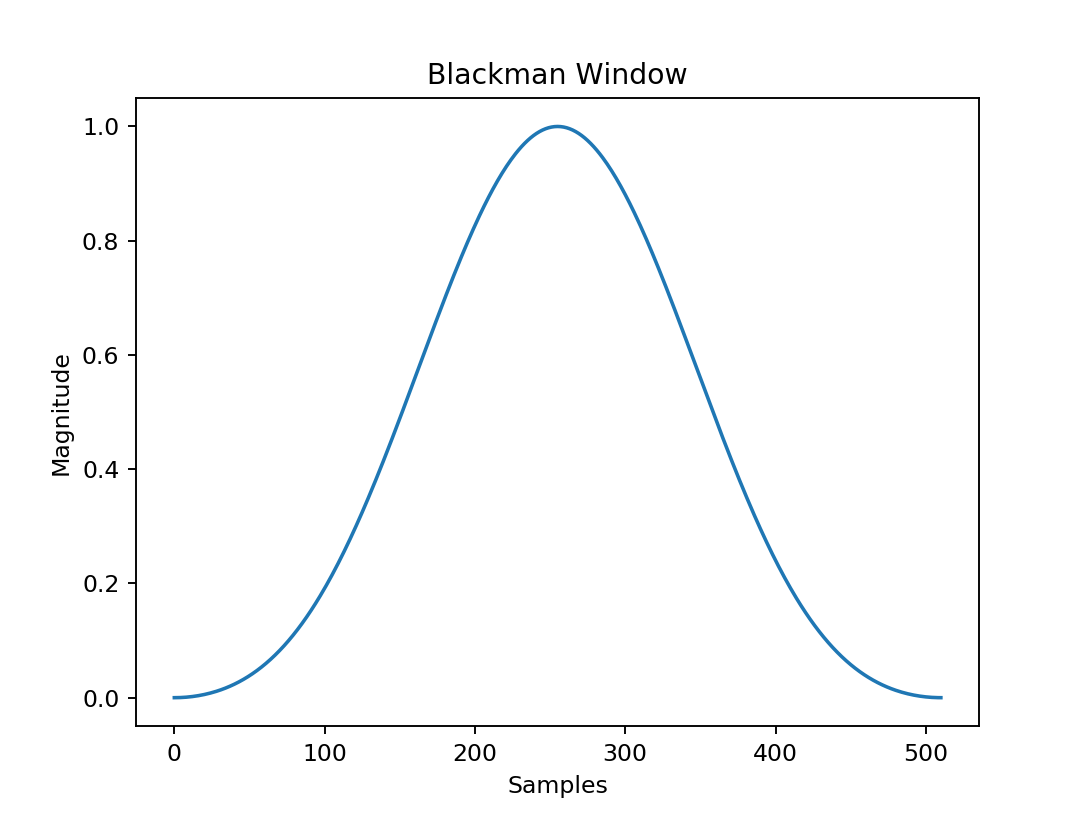
\includegraphics[width=0.6\textwidth]{blackman}
		\caption{Blackman window}
		\label{fig:blackman}
	\end{subfigure}
	\caption{Windows}
	\label{fig:windows}
\end{figure}

\paragraph*{} As you can see, the Hann window (\ref{fig:hann}) tapers a little less steeply than the Blackman window (\ref{fig:blackman}).
\clearpage

\begin{figure}[tb]
	\centering
	\begin{subfigure}[t]{\hsize}
		\centering
		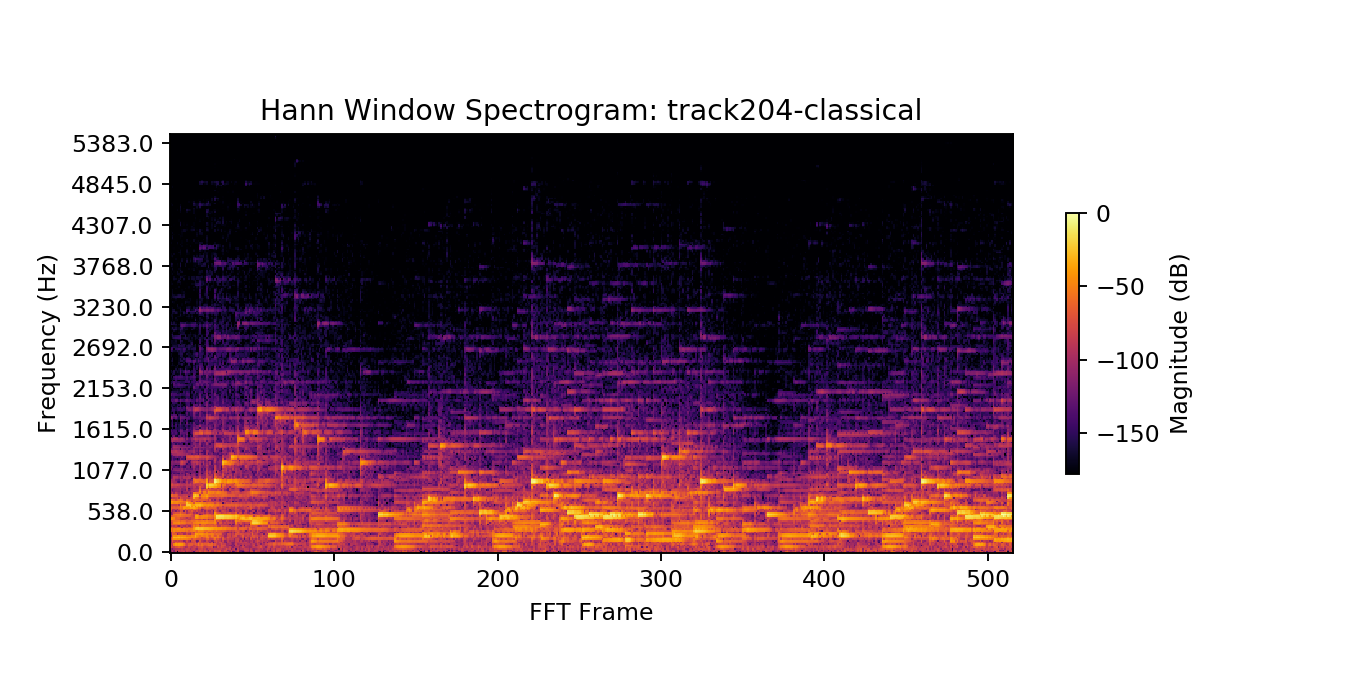
\includegraphics[width=0.9\textwidth]{powerHann_track204-classical}
		\caption{Spectrogram of 'track204-classical' using a Hann window}
		\label{fig:hann_classical}
	\end{subfigure}
	\begin{subfigure}[t]{\hsize}
		\centering
		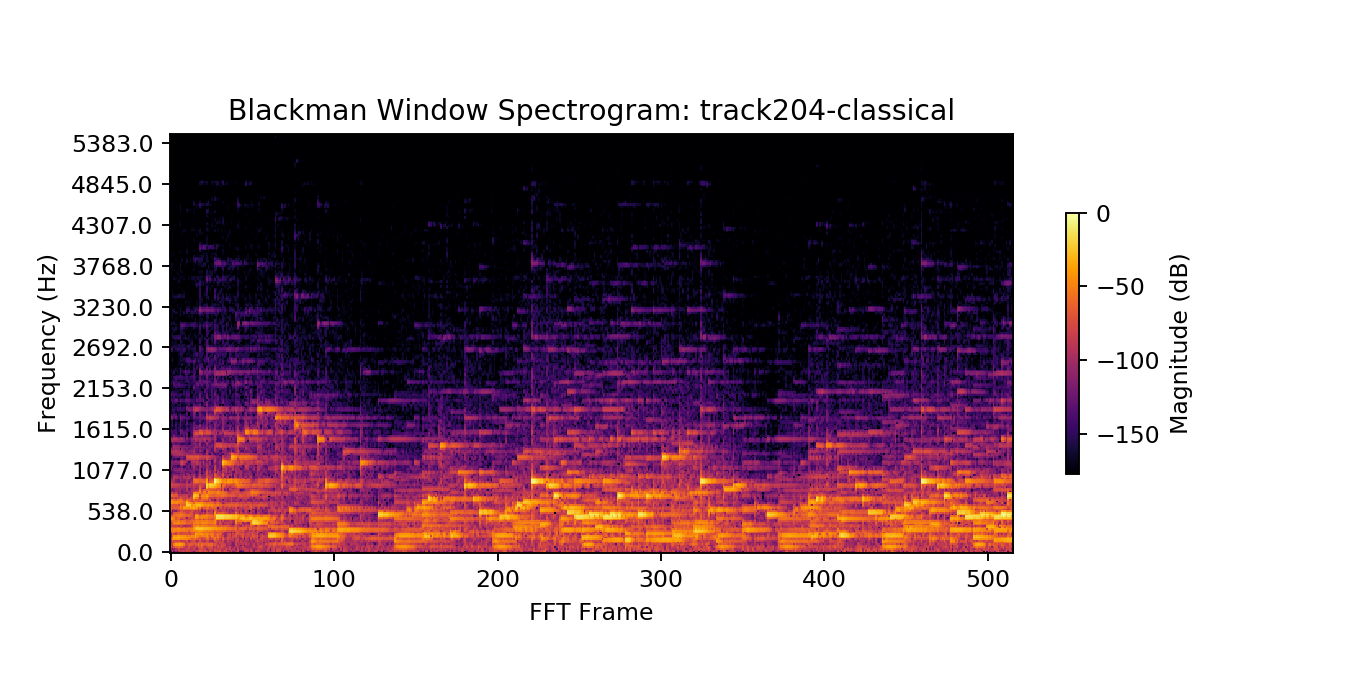
\includegraphics[width=0.9\textwidth]{powerBlack_track204-classical}
		\caption{Spectrogram of 'track204-classical' using a Blackman window}
		\label{fig:black_classical}
	\end{subfigure}
	\caption{Hann vs. Blackman windows for a classical music track}
	\label{fig:windows_classical}
\end{figure}
\clearpage

\begin{figure}[tb]
	\centering
	\begin{subfigure}[t]{\hsize}
		\centering
		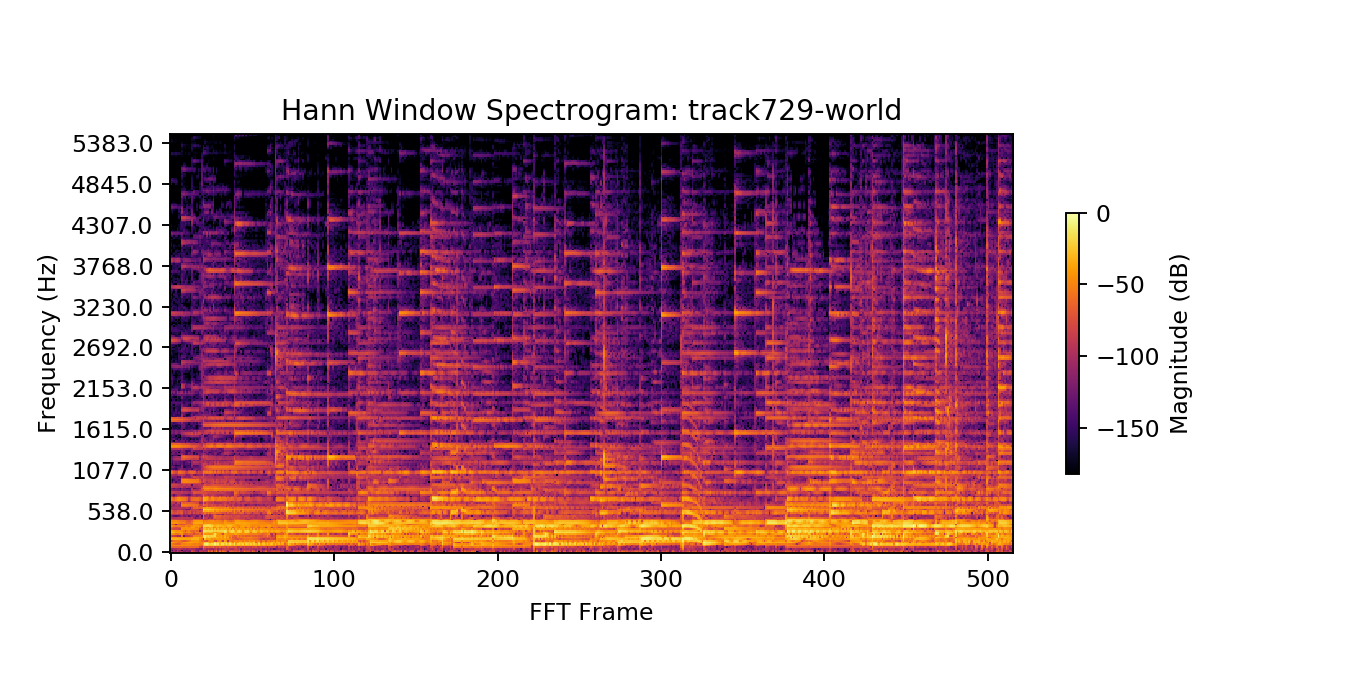
\includegraphics[width=0.9\textwidth]{powerHann_track729-world}
		\caption{Spectrogram of 'track729-world' using a Hann window}
		\label{fig:hann_world}
	\end{subfigure}
	\begin{subfigure}[t]{\hsize}
		\centering
		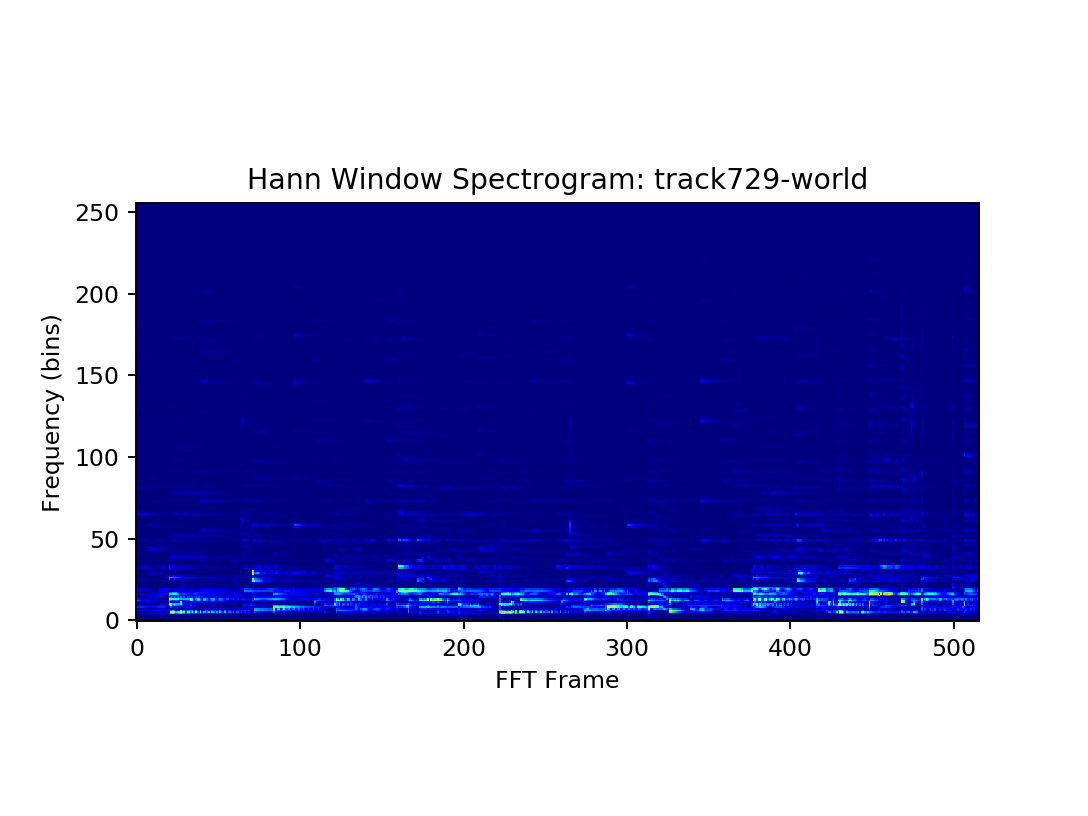
\includegraphics[width=0.9\textwidth]{powerBlack_track729-world}
		\caption{Spectrogram of 'track729-world' using a Blackman window}
		\label{fig:black_world}
	\end{subfigure}
	\caption{Loudness vs. frame}
	\label{fig:windows_world}
\end{figure}
\clearpage

\paragraph{Comments} As far as I can tell, the two spectrograms produced by these two windows in figures \ref{fig:windows_classical} and \ref{fig:windows_world} are identical. We will proceed with analysis using only the Blackman window.

\subsection{Spectral Centroid and Spread}
\paragraph*{} We wish to find the 'center of mass' of each frame in a spectrogram and will call this the spectral centroid. The centroid can be used to quantify sound sharpness or brightness. Additionally, we would like to find the spectral spread, or width of the spectrum around the centroid. Thus, we can then compare tone-like and noise-like sounds. For these concepts, we will treat the normalized magnitude of a spectral coefficient as if it were a 'probability' of that particular frequency. Then, for frame $n$, we have the 'probability' of frequency $k$

\begin{equation}
P_n(k) = \frac{|X_n(k)|}{\sum_{l=0}^{K} |X_n(l)|}
\end{equation}

Which we can then use to define the spectral centroid as

\begin{equation}
\mu_n = \sum_{k=0}^{K} kP_n(k)
\end{equation}

And the spectral spread for frame $n$ is the standard deviation given by

\begin{equation}
\sigma_n = \sqrt{\sum_{k=0}^{K} [k-\mu_n]^2 P_n(k)}
\end{equation}

The spectral centroid and spread were calculated for a classical, jazz, and metal song and a time-domain plot is shown in figure %\ref{fig:cs}.

\pagebreak

\begin{figure}[tb]
	\centering
	\begin{subfigure}[t]{\hsize}
		\centering
		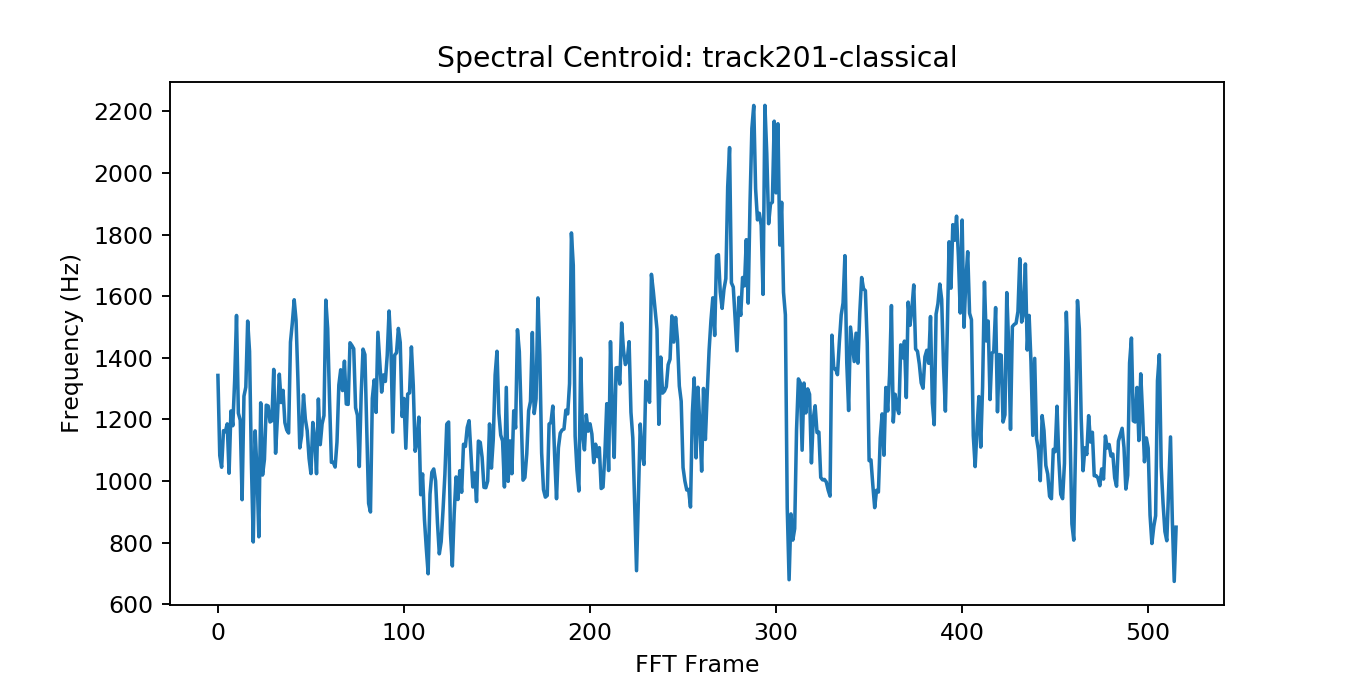
\includegraphics[width=0.9\textwidth]{centroid_track201-classical}
		\caption{Spectral centroid of 'track201-classical' as a function of frame number.}
		\label{fig:centroid_classical}
	\end{subfigure}
	\begin{subfigure}[t]{\hsize}
		\centering
		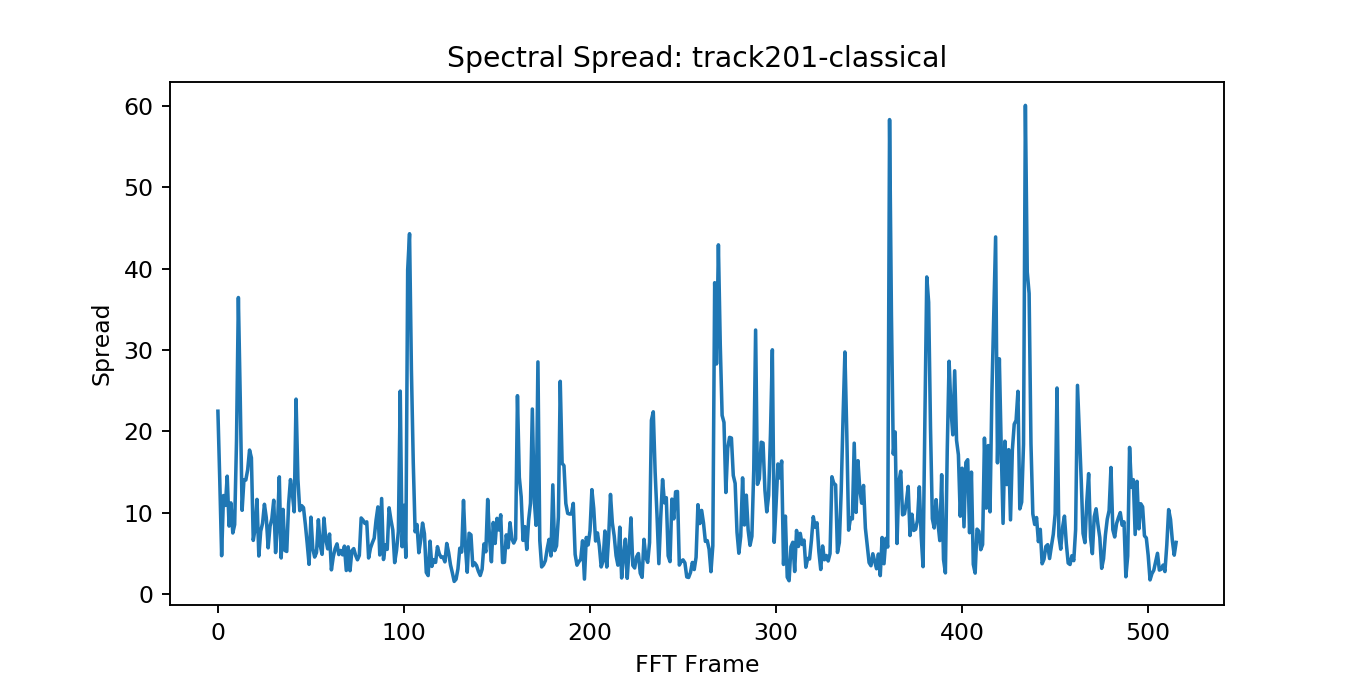
\includegraphics[width=0.9\textwidth]{spread_track201-classical}
		\caption{Spectral spread of 'track201-classical' as a function of frame number.}
		\label{fig:spread_classical}
	\end{subfigure}
	\caption{Centroid and spread \label{fig:cs}}
\end{figure}
\clearpage

\begin{figure}[tb]\ContinuedFloat
	\begin{subfigure}[t]{\hsize}
		\centering
		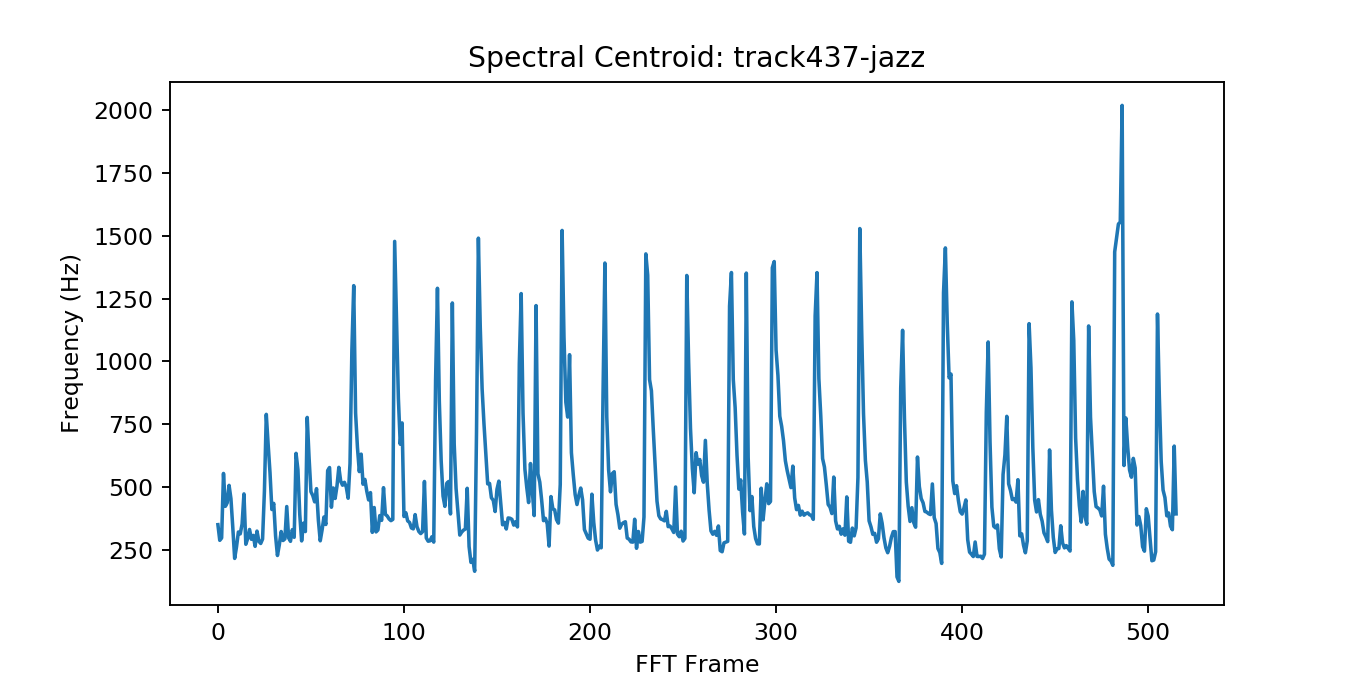
\includegraphics[width=0.9\textwidth]{centroid_track437-jazz}
		\caption{Spectral centroid of 'track437-jazz' as a function of frame number.}
		\label{fig:centroid_jazz}
	\end{subfigure}
	\begin{subfigure}[t]{\hsize}
		\centering
		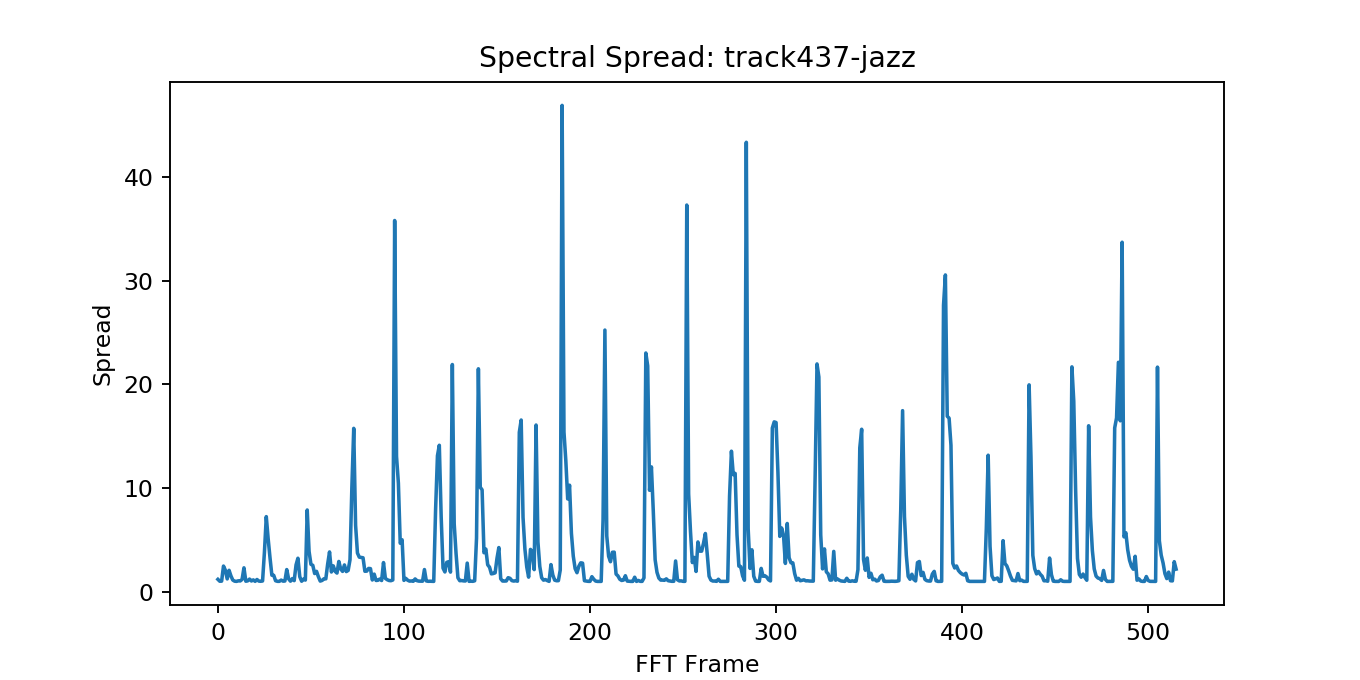
\includegraphics[width=0.9\textwidth]{spread_track437-jazz}
		\caption{Spectral spread of 'track437-jazz' as a function of frame number.}
		\label{fig:spread_metal}
	\end{subfigure}
	\caption{Centroid and spread}
\end{figure}
\clearpage

\begin{figure}[tb]\ContinuedFloat
	\begin{subfigure}[t]{\hsize}
		\centering
		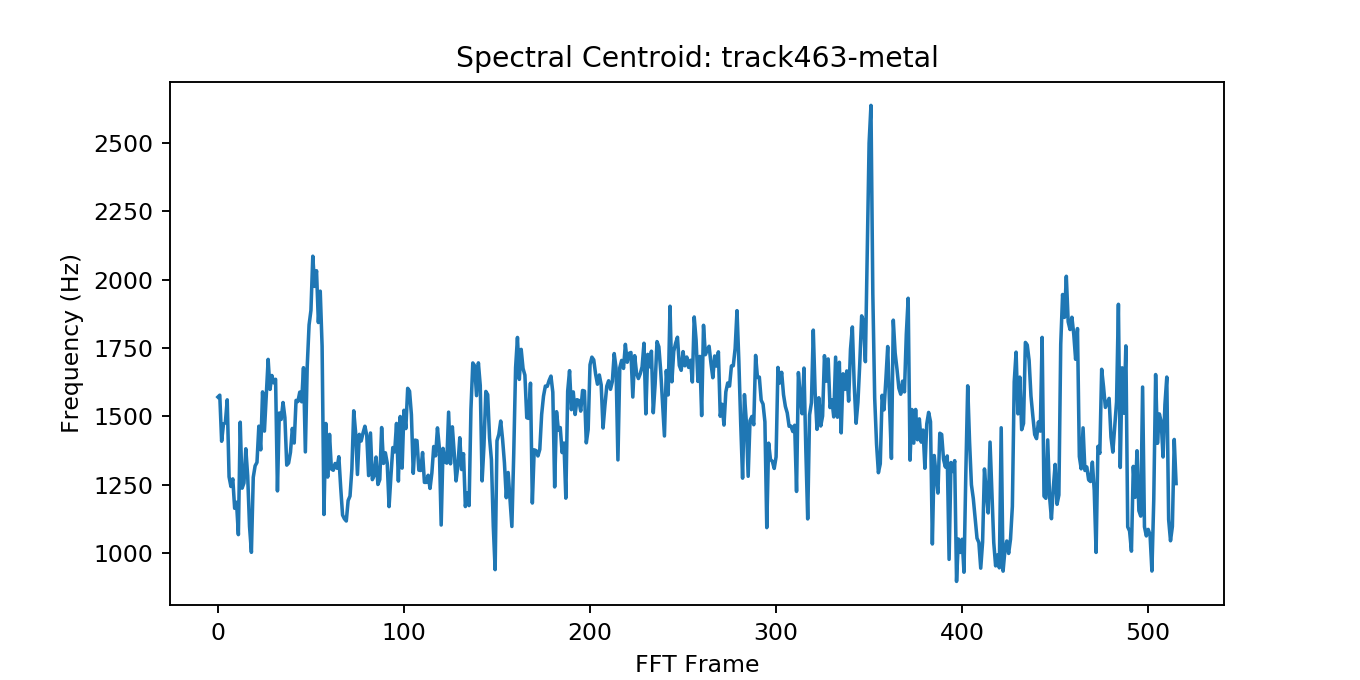
\includegraphics[width=0.9\textwidth]{centroid_track463-metal}
		\label{fig:centroid_metal}
		\caption{Spectral centroid of 'track463-metal' as a function of frame number.}
	\end{subfigure}
	\begin{subfigure}[t]{\hsize}
		\centering
		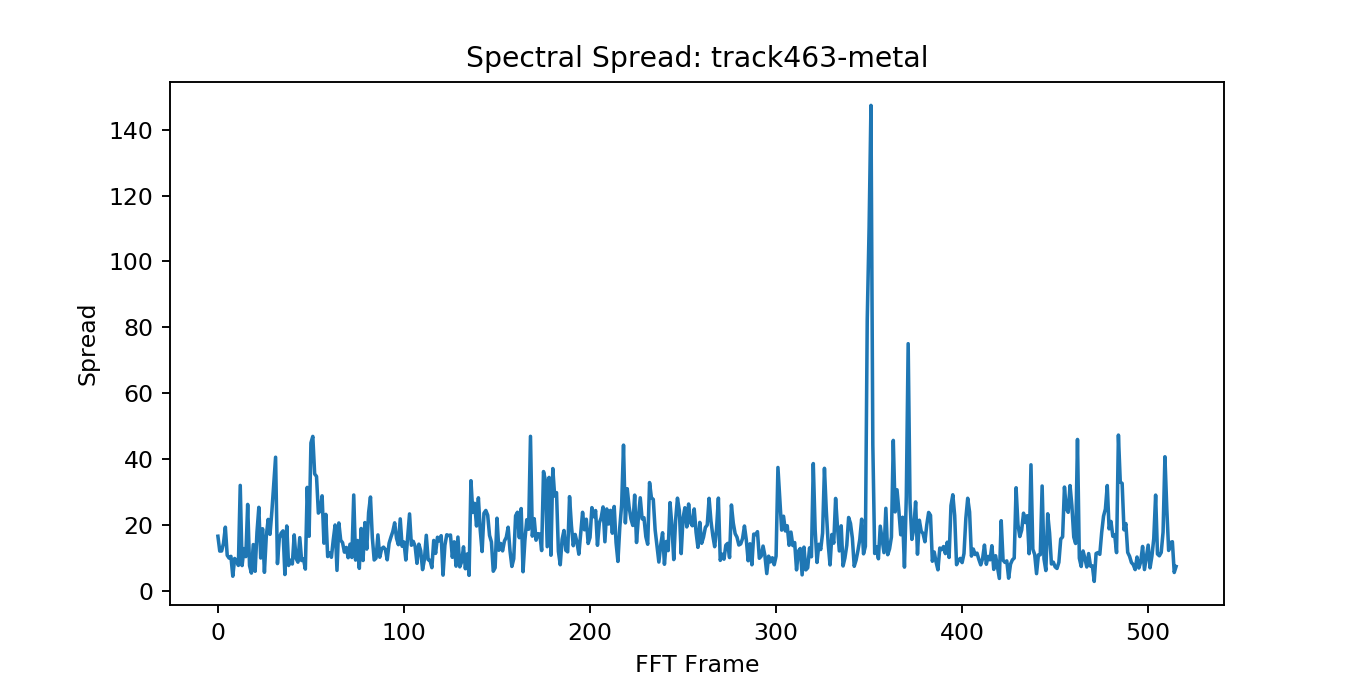
\includegraphics[width=0.9\textwidth]{spread_track463-metal}
		\caption{Spectral spread of 'track463-metal' as a function of frame number.}
		\label{fig:spread_metal}
	\end{subfigure}
	\caption{Centroid and spread}
\end{figure}
\clearpage



\end{document}

